%!TEX root = ../article.tex

% A new section
\section{Solution}
\label{sec:solution}
% Overview about the solution
% Types of users
% For each one, who he is, what he does...
% What was implemented for each one
The main goal of our solution is to assist
the development proximity-based mobile applications.
There are already some tools available for this purpose (presented in section \ref{sec:related_work}).
However, some of them are attached to a given platform, that is, developers
need to write one proximity-based application for each platform they want
to reach.
In order to circumvent this limitation, this solution allows developers
to use the same technologies that are used for any web application, such as \gls{HTML}, \gls{CSS} and Javascript.

Before starting the description of our solution, we need to take a look at three kinds of users that will be part of it:
\begin{itemize}
  \item End users: Anyone with a mobile device that installs an app to scan for nearby Smart Places;
  \item Owners: These users are the ones responsible for managing a given place that they want to turn into a Smart Place;
  \item Developers: The users that develop the code of the Smart Places.
\end{itemize}
% Introduce solution
% Smartphone
% App for owners
% App for users
% API for developers
% Beacons (Tags)
% Backend
Figure~\ref{fig:solution_overview} shows the main components of our solution, which are the following:
\begin{itemize}
  \item Beacons
  are the small devices that will act as tags, according to our definition of a Smart Place;
  \item Backend
  is where all the data is stored, that is, the Smart Places that are available, the Smart Places that each owner has configured, information about each beacon, etc;
  \item End Users Mobile App
  is another Android mobile app that allows users, with a mobile device, \gls{BLE} enabled, to have access to nearby Smart Places and to detect the beacons that belong to those Smart Places;
  \item Owners Mobile App
  is an Android mobile app that owners use to select which Smart Places they want to configure. It also allows to configure each individual beacon that belongs to a given Smart Place;
  \item Developers \gls{API} provides the necessary methods that developers can use to create their proximity-based services, based on the concept of a Smart Place.
\end{itemize}

\begin{figure}[!ht]
  \centering
    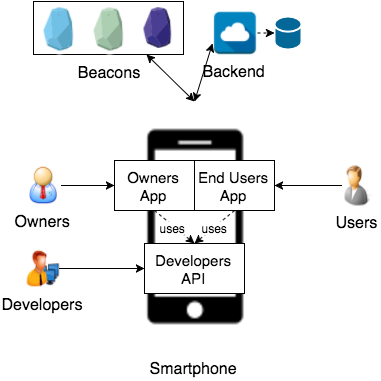
\includegraphics[width=0.4\textwidth, keepaspectratio]{figures/smart_places_solution_overview}
    \caption[Solution Overview]{Overview with the main components of our solution}
    \label{fig:solution_overview}
\end{figure}

Smart Places solution has a component that targets each one of the presented type of user.
Owners have a mobile app that allow them to turn the places they manage into Smart Places.
There is another mobile app to allow anyone, with a mobile device, such as a smartphone, to use the services provided by Smart Places nearby.
To develop these services our solution offers an \gls{API} that developers can integrate in their web applications to make them react to the presence of the user.

To create the backend, we have used Parse\footnote{http://parse.com} \gls{BaaS}. A \gls{BaaS} is a particular type of Software as a Service, that allows developers to specify which entities and their fields, that they need to store.
An \gls{BaaS} allows developers to not have to be concerned about aspects related to distributed systems, such as, scalability and security.
Since our backend only needs to be able to store and retrieve data, we chose this solution instead of doing an implementation of a \gls{REST} \gls{API} from the scratch.

Anyone that have a mobile device, such as a smartphone, can use the services provided by any Smart Place.
In our solution, there is an Android app, that notifies the user when he is nearby any Smart Place.
When the mobile device approaches any Smart Place, the app notifies the user that he is near a Smart Place.
When the user touches these notifications, the app shows an embedded web browser that contains a web page that can react to nearby objects, that is, beacons with meaning to the application.

The Smart Place owners manage one or more places where they want to provide some service to visitors, in their mobile devices.
In order to make owners be able to offer this kind of services, an Android app, designed for them, is offered by this solution.
This app offers features, such as, get a list of all available Smart Places and configure an instance of a Smart Place.
In order to configure a Smart Place, first, owners need to tag physical objects.
They need to deploy beacons in the right places.
Then, they use the mobile app to create an instance of a Smart Place following a small set of steps.
First, the app shows a list of all available Smart Places.
Then, the owner selects one and he can see a text explaining what that Smart Place is about.
Finnaly, the owner just needs to type a title and a message, that will appear in the users' mobile devices notifications when they are nearby

Owners configure the data of a Smart Place and end users, who are anyone with a mobile device and the app, can interact with objects nearby.
But, who will add behavior to these Smart Places, this kind of apps that can react to nearby objects with special tags?
Our solution offers a way for developers to create their Smart Places.
Also, we want to avoid the user having to install one mobile app for each Smart Place.
This is way, the app for end users,
has an embedded web browser, so they can use any Smart Place, as they would use any web application, without the need to install one more mobile app.
That is why a Javascript library is part of our solution.
This way, an existing web application can use this library and make it react to nearby objects tagged with \gls{BLE} beacons.
The library was turned into an open-source project, hosted on a github repository\footnote{http://github.com/samfcmc/smartplaces-js} and it is available, to install, using bower\footnote{http://bower.io}, which is a tool to manage frontend dependencies in web applications.
Then, developers just need to include the library and use the available functions.
The library is event-based, that is, the mobile apps, for owners and end users, emit events to the library, such as, a nearby beacon is detected, to the web application running inside a embedded web browser.
In this library, there is a global object, which is ``SmartPlaces'' with several methods.
All those methods need to receive a callback because, as already mentioned, the library follows an event-based approach.

We have created two examples of Smart Places, the Smart Restaurant and Smart Museum.
The Smart Restaurant allows customers of a restaurant to place their orders without the need to wait.
The Smart Museum allows museum's visitors to have access to more information, in their mobile devices, about a given object in an enxhibition, when they are in the proximity of that object.
We first built the Smart Restaurant.
While builiding this example, we wrote Javascript code to handle the events emitted by the mobile apps for owners and end users.
From this code, it was possible to create a library that resulted in a complete independent project, from which, the examples depend on.
After building the first example, we developed another one, which is the Smart Museum.
We defined the Javascript library as a dependency and observed that the same \gls{API} that fits the Smart Restaurant example, also could be used in the other example.
